% !TeX spellcheck = da_DK
\documentclass[12pt,fleqn]{article}

\usepackage[danish]{babel}
\usepackage{SpeedyGonzales}
\usepackage{MediocreMike}
%\usepackage{Blastoise}

\title{}
\author{Asger Schultz}
\date{\today}

\fancypagestyle{plain}
{
	\fancyhf{}
	\rfoot{Side \thepage{} af \pageref{LastPage}}
	\renewcommand{\headrulewidth}{0pt}
}
\pagestyle{fancy}
\fancyhf{}
\lhead{Asger Schultz}
\chead{}
\rhead{}
\rfoot{Side \thepage{} af \pageref{LastPage}}

\graphicspath{{Billeder/}}
\linespread{1.15}


%\numberwithin{equation}{section}
%\numberwithin{footnote}{section}
%\numberwithin{figure}{section}
%\numberwithin{table}{section}

\begin{document}

\maketitle
%\thispagestyle{fancy}
%\tableofcontents
-- 
\tableofcontents
\newpage 
\section{Data}
--


\section{Methods and analysis}
\subsection{Recommended measure}
-- Correlation and corr test\\
-- Fit of Michaelis-Menten model\\
-- Consider 
\subsection{Yield influence of bioavailability}
--ANCOVA using DGT and location\\
--ANCOVA using olsenP and location
\section{Results}
\begin{figure}[H]
	\centering
	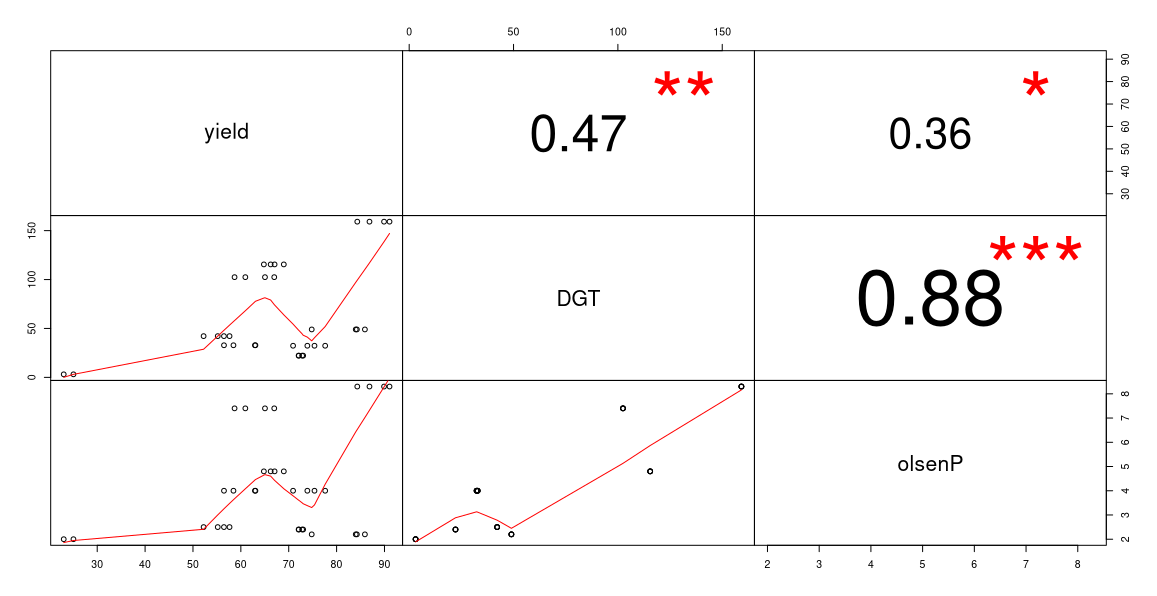
\includegraphics[width=.9\linewidth]{p2_corrplot}
	\caption{Visualization of a Correlation Matrix. On top the (absolute) value of the correlation plus the result of the cor.test as stars. On bottom, the bivariate scatterplots, with a fitted line}
\end{figure}
\begin{figure}[H]
	\centering
	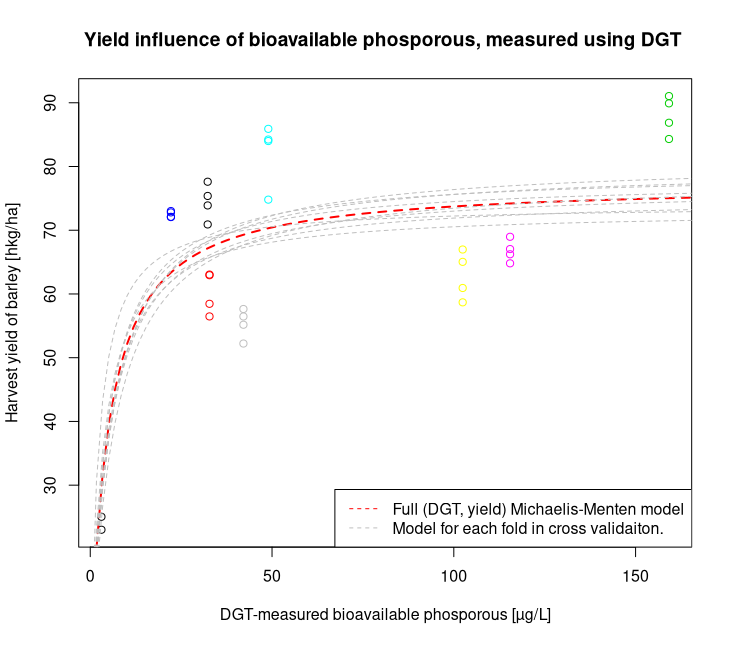
\includegraphics[width=.8\linewidth]{dgt_mmm}
\end{figure}
\begin{figure}[H]
	\centering
	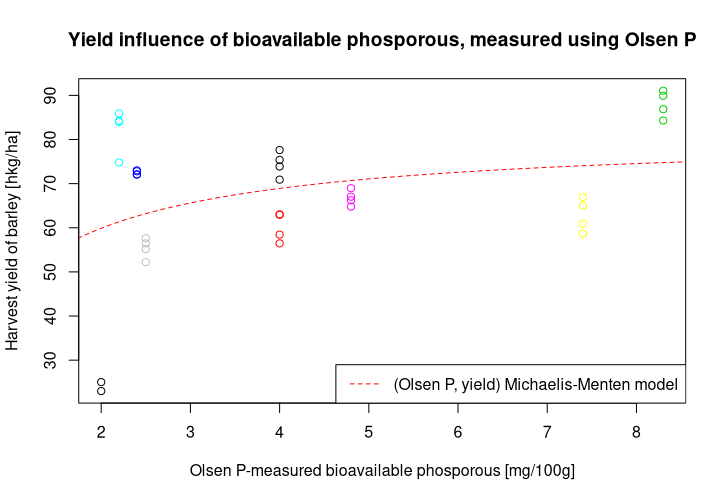
\includegraphics[width=.8\linewidth]{oP_mm}
\end{figure}

\begin{align*}
	& \sqrt{MSE_{dgt}}	 = 10.84
	&& \sqrt{MSE_{olsenP}} = 14.65
\end{align*}
%\begin{figure}[H]
%	\centering
%	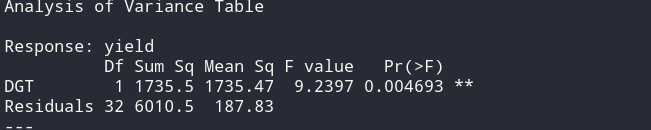
\includegraphics[width=.7\linewidth]{simpleDGT}
%\end{figure}



%\begin{figure}[H]
%	\centering
%	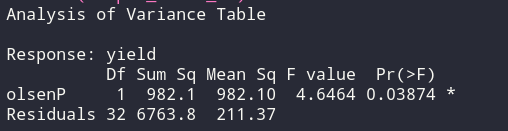
\includegraphics[width=.7\linewidth]{simpleOP}
%\end{figure}
\begin{figure}[H]
	\centering
	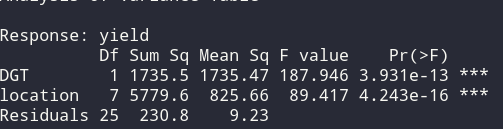
\includegraphics[width=.7\linewidth]{anovaDGT}
\end{figure}
\begin{figure}[H]
	\centering
	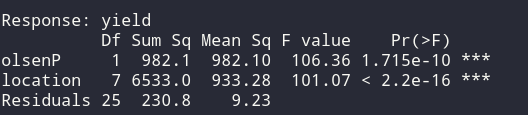
\includegraphics[width=.7\linewidth]{anovaOP}
\end{figure}

\section{Discussion}

\end{document}

















